%\documentclass[handout]{ximera}
\documentclass[nooutcomes]{ximera}

\usepackage{gensymb}
\usepackage{tabularx}
\usepackage{mdframed}
\usepackage{pdfpages}
%\usepackage{chngcntr}

\let\problem\relax
\let\endproblem\relax

\newcommand{\property}[2]{#1#2}




\newtheoremstyle{SlantTheorem}{\topsep}{\fill}%%% space between body and thm
 {\slshape}                      %%% Thm body font
 {}                              %%% Indent amount (empty = no indent)
 {\bfseries\sffamily}            %%% Thm head font
 {}                              %%% Punctuation after thm head
 {3ex}                           %%% Space after thm head
 {\thmname{#1}\thmnumber{ #2}\thmnote{ \bfseries(#3)}} %%% Thm head spec
\theoremstyle{SlantTheorem}
\newtheorem{problem}{Problem}[]

%\counterwithin*{problem}{section}



%%%%%%%%%%%%%%%%%%%%%%%%%%%%Jenny's code%%%%%%%%%%%%%%%%%%%%

%%% Solution environment
%\newenvironment{solution}{
%\ifhandout\setbox0\vbox\bgroup\else
%\begin{trivlist}\item[\hskip \labelsep\small\itshape\bfseries Solution\hspace{2ex}]
%\par\noindent\upshape\small
%\fi}
%{\ifhandout\egroup\else
%\end{trivlist}
%\fi}
%
%
%%% instructorIntro environment
%\ifhandout
%\newenvironment{instructorIntro}[1][false]%
%{%
%\def\givenatend{\boolean{#1}}\ifthenelse{\boolean{#1}}{\begin{trivlist}\item}{\setbox0\vbox\bgroup}{}
%}
%{%
%\ifthenelse{\givenatend}{\end{trivlist}}{\egroup}{}
%}
%\else
%\newenvironment{instructorIntro}[1][false]%
%{%
%  \ifthenelse{\boolean{#1}}{\begin{trivlist}\item[\hskip \labelsep\bfseries Instructor Notes:\hspace{2ex}]}
%{\begin{trivlist}\item[\hskip \labelsep\bfseries Instructor Notes:\hspace{2ex}]}
%{}
%}
%% %% line at the bottom} 
%{\end{trivlist}\par\addvspace{.5ex}\nobreak\noindent\hung} 
%\fi
%
%


\let\instructorNotes\relax
\let\endinstructorNotes\relax
%%% instructorNotes environment
\ifhandout
\newenvironment{instructorNotes}[1][false]%
{%
\def\givenatend{\boolean{#1}}\ifthenelse{\boolean{#1}}{\begin{trivlist}\item}{\setbox0\vbox\bgroup}{}
}
{%
\ifthenelse{\givenatend}{\end{trivlist}}{\egroup}{}
}
\else
\newenvironment{instructorNotes}[1][false]%
{%
  \ifthenelse{\boolean{#1}}{\begin{trivlist}\item[\hskip \labelsep\bfseries {\Large Instructor Notes: \\} \hspace{\textwidth} ]}
{\begin{trivlist}\item[\hskip \labelsep\bfseries {\Large Instructor Notes: \\} \hspace{\textwidth} ]}
{}
}
{\end{trivlist}}
\fi


%% Suggested Timing
\newcommand{\timing}[1]{{\bf Suggested Timing: \hspace{2ex}} #1}




\hypersetup{
    colorlinks=true,       % false: boxed links; true: colored links
    linkcolor=blue,          % color of internal links (change box color with linkbordercolor)
    citecolor=green,        % color of links to bibliography
    filecolor=magenta,      % color of file links
    urlcolor=cyan           % color of external links
}

\title{There Are Many Factors to Consider}
\author{Bart Snapp and Brad Findell}

\outcome{Learning outcome goes here.}

\begin{document}
\begin{abstract}
  We count the number of factors of an integer.
\end{abstract}
\maketitle

\label{A:CF}

Suppose we want to know how many factors $43,560$ has, but we don't need to list them all.  In this activity we develop a method for computing the number of factors of a number.  

\begin{teachingnote}
Maybe begin by asking student to list all the factors of $43,560$, in hopes that they will feel compelled to find a more efficient strategy.
\end{teachingnote}

\begin{problem}
Vic listed the following factors of 80:  1, 2, 4, 5, 8, 10, 20, 40, 80.  What is missing? Describe your method of checking the list.  
\vspace{0.2in}
\begin{teachingnote}
We hope they are organizing the factors in pairs and that they notice the $5$ has no ``partner.''  
\end{teachingnote}
\end{problem}

\begin{problem} Factors of 60. 
\begin{enumerate}
\item List the factors of 60. 
\vspace{0.2in}
\item Describe your method for ensuring that you have found all of the factors. 
\vspace{0.2in}
\begin{teachingnote}
Students are likely to test 1, 2, 3, 4, \dots.  If they list the factors in pairs, they should know they are done shortly after $6\cdot10$. 
\end{teachingnote}
\item Consider the prime factorization of 60 and the prime factorization of each of the factors.  Describe what you notice.   
\vspace{0.2in}
\begin{teachingnote}
Informally, the prime factorization of each factor of $60$ is ``included'' in the prime factorization of $60$.  Since $60=2^2\cdot 3\cdot5$, the factors can use only the primes $2$, $3$, and $5$, and with an exponent less than or equal to its exponent in $60$.  
\end{teachingnote}
\end{enumerate}
\end{problem}

\begin{problem}
Factors of $3^7$.  
\begin{enumerate}
\item Is $2$ a factor of $3^7$?  Say how you know. %What about $7$?  What about $6$? 
\vspace{0.2in}
\item Is $7$ a factor of $3^7$?  Say how you know. 
\vspace{0.2in}
\item List all the factors of $3^7$. 
\vspace{0.2in}
\item Generalize: If $p$ is a prime number, how many factors does $p^n$ have?  Explain your reasoning.  
\vspace{0.2in}
\begin{teachingnote}
Answer: $(n+1)$.
\end{teachingnote}
\end{enumerate} 
\end{problem}

\begin{problem} 
List all the factors of $3^2\cdot7^3$.  Use your example to reason about the number of factors of $p^nq^m$, where $p$ and $q$ are both prime numbers.  
\vspace{1.5in}
\begin{teachingnote}
Students are likely to list $1$, $3$, $7$, $3^2$, $7^2$, and others.  But the challenge here is developing a systematic way of ensuring that all are listed.  One way to get started is to say, ``Can you list all of the factors that have exactly one 3?''  Then students will list $3$, $3\cdot7$, $3\cdot7^2$, and $3\cdot7^3$.  What about $3$ to other powers?  

A general strategy: Fix the exponent of 3 and list all of the possible exponents of 7 that fit with it.  Now try a different exponent of 3.  Were we systematic in trying all of the exponents of 3?  

Answer: $(n+1)(m+1)$.
\end{teachingnote}
\end{problem}

\begin{problem} 
List all the factors of $3^2\cdot7^3\cdot11$.  Use your example to reason about the number of factors of $p^nq^mr^s$, where $p$, $q$, and $r$ are all prime numbers.  
\vspace{1.5in}
\begin{teachingnote}
Answer: $(n+1)(m+1)(r+1)$.
\end{teachingnote}
\end{problem}

\begin{problem}
How many factors does $43,560$ have?  Use the example of $43,560$ to describe and explain a method for computing the number of factors that a
number has.
\end{problem}
\vspace{1.5in}

%\begin{problem} Which integers between $0$ and $100$ have the most factors?         
%\end{problem}

%\begin{problem}
%Consider the following diagram:
%\[
%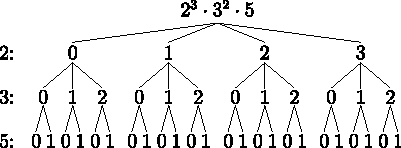
\includegraphics{../graphics/treeDia.pdf}
%\]
%What is going on in this diagram? What do the numbers represent? How
%does it help you count the number of factors of $2^3\cdot 3^2 \cdot
%5$?
%\end{problem}

\end{document}
